%%%%%%%%%%%%%%%%%%%%%%%%%%%%%%%%%%%%%%%%%
% Journal Article
% LaTeX Template
% Version 1.3 (9/9/13)
%
% This template has been downloaded from:
% http://www.LaTeXTemplates.com
%
% Original author:
% Frits Wenneker (http://www.howtotex.com)
%
% License:
% CC BY-NC-SA 3.0 (http://creativecommons.org/licenses/by-nc-sa/3.0/)
%
%%%%%%%%%%%%%%%%%%%%%%%%%%%%%%%%%%%%%%%%%

%----------------------------------------------------------------------------------------
%	PACKAGES AND OTHER DOCUMENT CONFIGURATIONS
%----------------------------------------------------------------------------------------

\documentclass[twoside]{article}

\usepackage{lipsum} % Package to generate dummy text throughout this template

\usepackage[sc]{mathpazo} % Use the Palatino font
\usepackage[T1]{fontenc} % Use 8-bit encoding that has 256 glyphs
\linespread{1.05} % Line spacing - Palatino needs more space between lines
\usepackage{microtype} % Slightly tweak font spacing for aesthetics
\usepackage{paralist}
\usepackage[margin={1.5cm,1.5cm},top=32mm,columnsep=20pt]{geometry} % Document margins
\usepackage{multicol} % Used for the two-column layout of the document
\usepackage[hang, small,labelfont=bf,up,textfont=it,up]{caption} % Custom captions under/above floats in tables or figures
\usepackage{booktabs} % Horizontal rules in tables
\usepackage{graphicx,float}
\usepackage{float} % Required for tables and figures in the multi-column environment - they need to be placed in specific locations with the [H] (e.g. \begin{table}[H])
\usepackage{hyperref} % For hyperlinks in the PDF
\usepackage{amsmath,amsfonts,amsthm}
\usepackage{lettrine} % The lettrine is the first enlarged letter at the beginning of the text
\usepackage{paralist} % Used for the compactitem environment which makes bullet points with less space between them
\usepackage{subfigure}% For side by side figure

\usepackage{abstract} % Allows abstract customization
\renewcommand{\abstractnamefont}{\normalfont\bfseries} % Set the "Abstract" text to bold
\renewcommand{\abstracttextfont}{\normalfont\small\itshape} % Set the abstract itself to small italic text
\usepackage[toc,page]{appendix}

\usepackage{algorithm}
\usepackage[noend]{algpseudocode}
\makeatletter
\def\BState{\State\hskip-\ALG@thistlm}
\makeatother

\usepackage{titlesec} % Allows customization of titles
\renewcommand\thesection{\arabic{section}} % Roman numerals for the sections
\renewcommand\thesubsection{\arabic{subsection}} % Roman numerals for subsections
\titleformat{\section}[block]{\Large\scshape\centering}{\thesection.}{1em}{} % Change the look of the section titles
\titleformat{\subsection}[block]{\large}{\thesection.\thesubsection.}{1em}{} % Change the look of the section titles

\usepackage{fancyhdr} % Headers and footers
\pagestyle{fancy} % All pages have headers and footers
\fancyhead{} % Blank out the default header
\fancyfoot{} % Blank out the default footer
\fancyhead[C]{Userless Classification for the Yelp Dataset Challenge} % Custom header text
\fancyfoot[RO,LE]{\thepage} % Custom footer text

%----------------------------------------------------------------------------------------
%	TITLE SECTION
%----------------------------------------------------------------------------------------

\title{\vspace{-15mm}\fontsize{24pt}{10pt}\selectfont\textbf{Userless Classification for the Yelp Dataset Challenge}} % Article title

\author{
\large
\textsc{Nicolas Drizard \& Virgile Audi}\\[2mm] % Your name
\normalsize Final Project for CS281, Harvard University \\ % Your institution
\normalsize {nicolas.drizard@g.harvard.edu \quad vaudi@g.harvard.edu} % Your email address
\vspace{-5mm}
}
\date{}

%----------------------------------------------------------------------------------------

\begin{document}

\maketitle % Insert title

\thispagestyle{fancy} % All pages have headers and footers

%----------------------------------------------------------------------------------------
%	ABSTRACT
%----------------------------------------------------------------------------------------

\begin{abstract}

\noindent

Our objective is to improve the categorization system of the Yelp businesses using machine learning techniques. To achieve our goal, we extract significant information out of the text reviews posted on Yelp using our own coded-up Latent Dirichlet Allocation (LDA) using online variational inference (OVI), and benchmark it with the LDA using a Gibbs samplingmethod (GS) and the Non Negative Matrix Factorisation (NMF). We then present two methods for classifying restaurants. We first resorted to a supervised approach with one-vs-all classifiers on  the text reviews combined with characteristic features of businesses - such as localisations, prices, customer type or check-in counts. The second approach is unsupervised, using the Walktrap Algorithm, a community detection algorithm on network of restaurant. If the different feature extraction methods performs differently for the supervised and unsupervised approach, we observe some very promising results. The results could be used as the first step to an automated categorization system on the Yelp website. 

\end{abstract}

%----------------------------------------------------------------------------------------
%	ARTICLE CONTENTS
%----------------------------------------------------------------------------------------

\begin{multicols}{2} % Two-column layout throughout the main article text

\section{Introduction}

\lettrine[nindent=0em,lines=1]{T}he classification system in Yelp is manual. When the owner of a business creates a page for his restaurant or bar, he is can provide a certain number of labels. Yelp users can then alter or even add new tags based on their experiences. As part of the Yelp Data Set Challenge Round 6, we decided to tackle the issue of entries classification. Our ultimate objective is to create an automatised method to classify the businesses, based on their properties and most importantly on their reviews from Yelpers. \\

This project can be divided in three parts. First, to extract feature, we applied various dimensionality reduction methods such as Latent Dirichlet Allocation (LDA) or Non-negative Matrix Factorisation (NMF) to embed the reviews into a geometrical space. Then, we applied supervised learning methods to evaluate how relevant are the feature to predict the labels. Last, we built an unsupervised clustering method using the Walktrap algorithm.

%------------------------------------------------
\columnbreak
\section{Data}

Yelp provides data on all kinds of venues such as dentists or bars in 5 cities in the United-States and Europe. The data can be summarised as follows:

\begin{compactitem}
    \item 1.6 million reviews;
    \item 61 000 businesses;    
    \item 481 000 attributes; 
    \item 168 customer check-in counts, corresponding to the average number of checkins per hour per day of the week.
\end{compactitem}

\noindent For simplicity, we chose to focus on restaurants and bars in the city of Las Vegas, Nevada. This reduced the data to a dataset of 3822 businesses, with about 20 thousands reviews and 250 other features per entry such as hours, parking availabity, take-out, ambience. If the numerical data provided by Yelp is mostly cleaned, it was not the case of the text data. Cleaning the reviews represented a significant part of this final project. We present some of the steps we followed in the process:\\

\begin{compactitem}
    \item We aggregated all the reviews about a particular business into a "super" review, in order to get a general sense of what the restaurant was about;
    \item We applied spelling corrections, removed common stopwords and generic words such as "table" or "restaurants";
    \item We attempted at only selecting common words and not adjectives in order to focus on what the venues were about and not the users' opinions (this process was done taking advantage of Spark to reduce the computing time);
    \item We transformed the corpus of "super reviews" into a document-term matrix that we could exploit;
    \item As we aggregated the reviews, some words may be more prevalent than others, so we scaled the words counts into the range [0, 100] for each review.
\end{compactitem}

%------------------------------------------------

\section{Feature Extraction}

\subsection{Approach}

To extract content from the reviews, we applied two methods from topic modeling to reduce the document term matrix into meaningful information. We first looked at LDA, using both a Gibbs sampler (GS) and an Online Variational Inference (OVI) algorithm. Note that we used the Gibbs sampler as a way to benchmark our own version of OVI. The motivation behind OVI is twofold. First, it appeared more appropriate to the data we were working with, indeed new reviews can always be added to the corpus in continuous flow. Second, it showed some extremely significant time improvement over the Gibbs sampler version in Python. We also wanted to compare the performance of LDA with a non-probabilistic approach which is the NMF. 

\subsection{Latent Dirichlet Allocation}

The LDA is a three-level hierarchical Bayesian model. The basic idea is that documents are represented as random mixtures over latent topics and each topic is characterized by a distribution over words.\cite{LDA}\\


\noindent The generative process for a document \textbf{w} in a corpus D is the following:
\\
\begin{compactenum}
	\item Choose the topics representation:\newline $\phi \sim$ Dir($\beta$)
	\item Choose the number of words:\newline $ N \sim $ Poisson($ \xi $)
	\item Choose the distribution of topics:\newline $\theta_w \sim$ Dir($\alpha_w$)
	\item For each of the N words:
	\begin{compactenum}
		\item Choose a topic assignement:\newline $z_{n,w} \sim \text{Multinomial}(\theta_w)$
		\item Choose a word: \newline$w_n \sim \text{ Multinomial}(\phi_{z_{n,w}})$
	\end{compactenum}
\end{compactenum}

\begin{figure}[H]
\centering
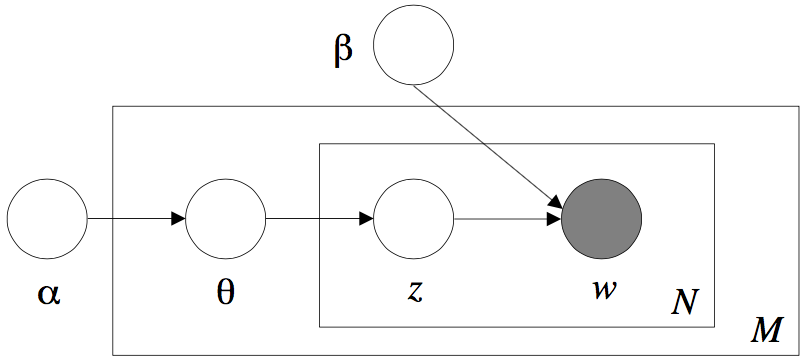
\includegraphics[width=0.8\linewidth]{img/LDA.png}
\caption{Graphical Model Representation of LDA}
\end{figure}

\subsection{Inference}

The main issue relies in computing the posterior distribution of the hidden variables given a document:\\

\begin{align*}
p(\theta, \mathbf{z} |\mathbf{w}, \alpha, \beta) = \frac{p(\theta, \mathbf{z}, \mathbf{w} | \alpha, \beta)}{p(\mathbf{w} | \alpha, \beta)}
\end{align*}

\noindent This distribution is intractable. As mentioned above, we used two  methods to infer it: through a Gibbs sampler or variational inference. In the first case, we are estimating the hyper parameters $\theta$ and $\phi$ with samples on the different variables. Alternatively, we chose the online variational inference method which finds the variational parameters that optimize a lower bound on the loglikelihood. The setup \cite{OLLD} of the variational inference is as follows. We first approximate the true posterior by a simpler and factorised distribution:

$$q(\boldsymbol{z},\boldsymbol{\theta},\boldsymbol{\beta}) = q(\boldsymbol{z})q(\boldsymbol{\theta})q(\boldsymbol{\beta}) $$ 

\noindent where:
$$ q(z_{di} = k) = \phi_{d_{w_{di}k}} \quad q(\theta_d) = \text{Dir}(\theta_d,\gamma_d) \quad q(\beta_k) = \text{Dir}(\beta_k,\lambda_k) $$

\noindent The $\boldsymbol{\gamma}$ parameter rule the topic assignments for each document and the $\boldsymbol{\lambda}$, the topics themselves. We then minimise the KL divergence between the distribution $q$ and the true posterior $p$. What differs in the online variational inference is that we sample a mini-batch of document at each step and perform the E-step as if this mini-batch constituted the entire corpus. We present the algorithm below:

\begin{algorithm}[H]
\caption{Minibatch Online Variational Inference}\label{euclid}
\begin{algorithmic}[1]
\State Define $\rho_t \equiv (\tau_0 + t)^{-\kappa}$
\State Initalise $\boldsymbol{\lambda}$ randomly
\State Sample a batch $\mathcal{S}$ of documents of size S
\For{$t$=0 to $|D|/|\mathcal{S}|$}
\For {$d$ in $\mathcal{S}$}
\While {$\gamma_(d)$ hasn't converged}
\State Set $\phi^{(d)}_{twk} \propto \exp\{\mathbb{E}_q\log\theta_{tk} + \mathbb{E}_q\log\beta_{kw}\}$
\State Set $\gamma^{(d)}_{tk} = \alpha + \sum_{w} \phi^{(d)}_{twk}n_{tw}$
\EndWhile
\State Compute $\tilde{\lambda}_{kw} = \eta +\frac{D}{S}n_{tw}\phi^{(d)}_{twk}$
\EndFor
\State $\boldsymbol{\lambda} = (1-\rho_t)\boldsymbol{\lambda}+\rho_t\boldsymbol{\tilde{\lambda}}$
\EndFor
\end{algorithmic}
\end{algorithm}

\noindent where $\kappa \in (0.5,1]$ rules how fast we forget old values of $\tilde{\lambda}$ and $\tau_{0}$ how much weight one wants to put on the first iterations. $\alpha$ and $\eta$ where fixed at the same value $\frac{1}{|D|}$.

\subsection{Evaluation Method}

We need a measure to evaluate the performance of our model and to tune the hyperparameters. We use the perplexity on held-out data as a measure of our model fit. The perplexity is defined as the geometric mean of the log likelihood of the words in the held-out set of documents given the trained model. In our case, for each document we held out 20\% of the words which constitue the validation set to apply a 5-fold cross-validation.

\begin{align*}
	perplexity(D_{test}) & = \frac{\sum\limits_{d \in D_{test}} \log p(words)}{\sum\limits_{d \in D_{test}}|d|}\\
	perplexity(D_{test}) & = \frac{\sum\limits_{d \in D_{test}} \sum\limits_{w \in d} \log \left( \sum_{t \in topics} p(w|t)p(t|d) \right)}{\sum\limits_{d \in D_{test}}|d|}
\end{align*}

\noindent We used this measure to optimize the number of topics K and the hyper parameters $\kappa$, $\tau$ of the optimization. We also used the perplexity on the training set to benchmark our algorithm with the Gibbs sampler in the LDA 1.0.3 package in Python:

$$\text{perp}_{OVI} = -6.78 \quad \text{and} \quad \text{perp}_{GS} = -6.45$$

\begin{figure}[H]
\centering
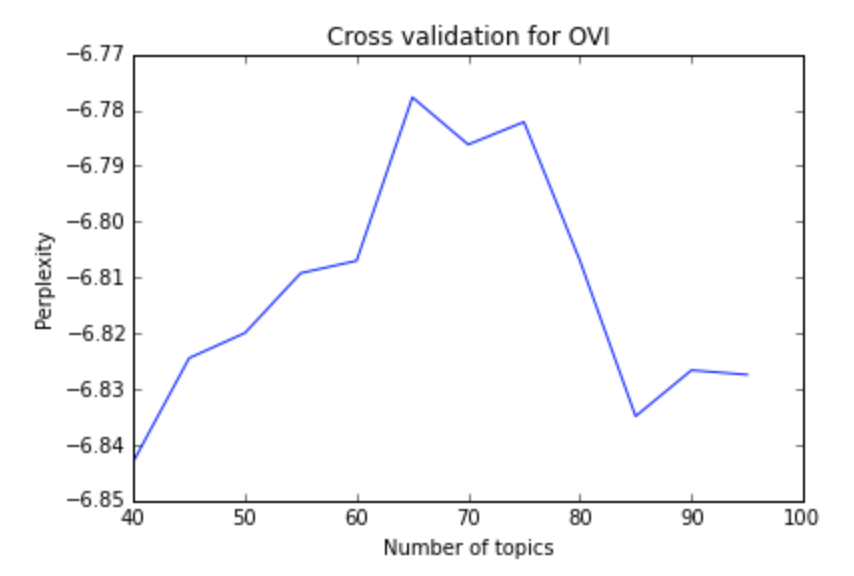
\includegraphics[width=1\linewidth]{img/V.png}
\caption{5-fold Cross Validation over the number of Topics}
\end{figure}

\subsection{Results}
Another way to assess the performance of our LDA was to inspect the topics outputted by the algorithm. We present some of the most significant topics:\\

\begin{figure}[H]
\centering
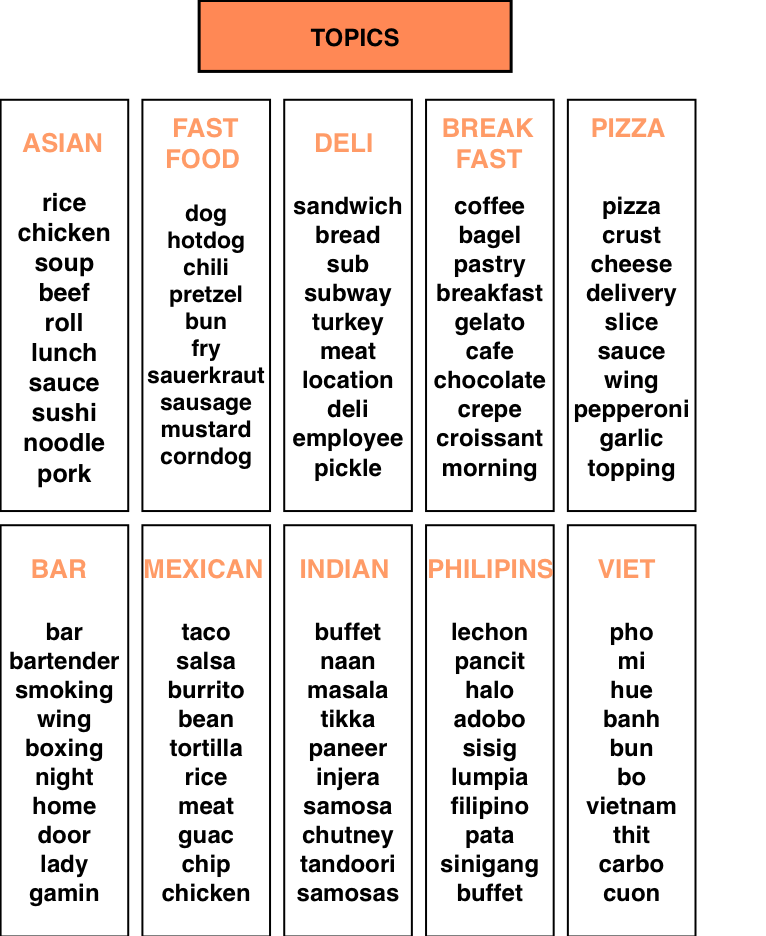
\includegraphics[width=1\linewidth]{img/topics.png}
\caption{Topics extracted from the Las Vegas reviews using OVI}
\end{figure} 

\noindent We obtained similar results using the NMF approach. The topics themselves were not our primary interested. As mentioned in the introduction, we were using these methods primarly for dimensional reduction purposes. \\

We would like to make a general comment about the online variational algorithm. We noticed that its algorithm is extremely sensitive to the hyperparametrisation, i.e the batch size $S$, the forgetfullness parameter $\kappa$ and the early iterations weith parameter $\tau$. This was also noted by Tamara Broderick, Nicholas Boyd, Andre Wibisono and Ashia C. Wilson in their paper\cite{svi}. In addition to validating the number of topics, validating over these parameters was crucial to obtain valuable results.\\

We now present two different approaches to answer the question of classification using supervised and unsupervised machine learning methods.\\

%------------------------------------------------
\section{Classification}

Once the features have been extracted, we can apply supervised learning methods to classify the Yelp restaurants considering the category labels as output. Several approaches are possible to solve this multi-label classiffication task depending on the nature and patterns of the features.

\subsection{Approach}

\noindent The features are divided into two main parts: on one hand, the topics assignements extracted from the reviews with the LDA and on the other hand, the properties provided by Yelp. Pre-processing the latter part provided a 198 dimensional vector. These features contained both numerical values (rating, space coordinates, number of reviews, customer check-in...) and categorical ones which we converted into indicator variables.\\

\noindent Given our numerical features, many different discriminative and generative models could be appllied on our data. Nonetheless, the indicator features are sparse and the data are really noisy. We therefore needed to consider a penalized or aggregated model to reduce overfitting.\\

\noindent We chose a one-vs-all approach to tackle this multi-label task, and built one binary classifier for each label. We then assign to the entries the labels predicted by each model. The goal is here to explore how the different models perform and to tune them to come up with the best estimator. We developped our own L2 penalized logistic regression and used \emph{scikit-learn} \cite{sklearn} for the other models.

\subsection{Results}

\paragraph{Dimensionality Reduction}

\noindent We decided to reduce the dimension of the dataset before fitting our model. As the high-dimensionality is largely due to the customer check-in counts and as they share a common structure, we decided to project them in an euclidean space. The combination of the embedded features with the latent features provided by the reviews is more consistent. We apply a principal component analysis (PCA) while keeping \textbf{95\%} of the variance which reduces the dimension from \textbf{168} to \textbf{19}.

\paragraph{Models Evaluation}

\noindent Here we provide the different results we obtained from our models. We ran one-vs-one classifiers for the 10 different labels which are the most represented in the Las Vegas restaurants. Then we evaluated for each classifier its accuracy and averaged them to get the evaluation metric printed in the table. We tested them on three different kinds of features provided by the reviews depending on the method used to build them. Then we ran each model on the PCA projection and on the raw data. We also show for comparaison the baseline model where we do not assign any label. This result is really high because of the skewness of the considered sample, among the 10 categories considered for 3822 restaurants the most represented (Fast Food) contains 553 entries and the least (American New) 280 entries.

\begin{figure}[H]
\begin{center}
    \begin{tabular}{| l | l | l | l |}
    \hline
    & OVI LDA & GS LDA & NMF \\ \hline
    Baseline: all False & 90,02 \% &  90.02 \% &  90.02 \% \\ \hline
    Kernel rbf SVM & 91.00\%  &  90.73\%  &  90.67\% \\ \hline
    Kernel rbf SVM + PCA & 90.62\%  &  90.85\%  &  90.85\% \\ \hline
    Logistic Regression & 91.39\%  &  91.86\%  &  91.86\%\\ \hline
    Logistic Regression + PCA & 92.37\%  &  92.89\%  &  93.16\% \\ \hline
    Lasso & 91.18\%  &  93.75\%  &  92.40\% \\ \hline
	Lasso + PCA & 92.53\%  &  \textbf{94.83}\%  &  93.35\% \\ \hline
    Random Forest & 92.12\% &  93.58\% &  93.37\% \\ \hline
    Random Forest + PCA & 92.84\% &  94.66 \% &  94.06\% \\ \hline
    \end{tabular}
\end{center}
\caption{Classification results for different features}
\end{figure}

\noindent The first outcome of this comparative study is the differences between each feature extraction method. The model built with the GS features seems to outperform on average the other two, which perform similarly to each other. These results are not surprising as the variationnal inference learns the closest model to the underlying one in terms of KL divergence. With the Gibbs sampling approach, we approximate the true underlying distribution at each iteration to refine our estimator. As a result, the latter method is by nature better to find the best model as long as it has enough iteration to converge and there actually exists an underlying mixture models. Nevertheless, the OVI remains a good proxy with regard to its time execution (53s against 50min for the Gibbs Sampler).\\

\noindent If we then compare the models to each other, we see that the support vector machine performs poorly and that the linear version was even closer to the baseline. This confirms that the data is not linearly separable and even their projection by the rbf function used in sklearn library (gamma function) is quite impossible to separate. The logistic regression performs better under the l1 penalization because of the sparsity of our features. Lastly, the random forest managed to reduce the common overfitting of the decision trees while aggregating them and provides on the PCA projection a very good estimator.\\

\noindent We plotted here the ROC curves of the Random forest for the 10 classes considered. The ranking with respect to the area under the curve is very close to the one induced by the number of positive elements for each class.This shows that the more positive elements we have, the better the model actually performs. Nonetheless, trying to learn the model on a smaller and more balanced train set for the classes with a low number of positive elements does not improve the classification accuracy.

\begin{figure}[H]
	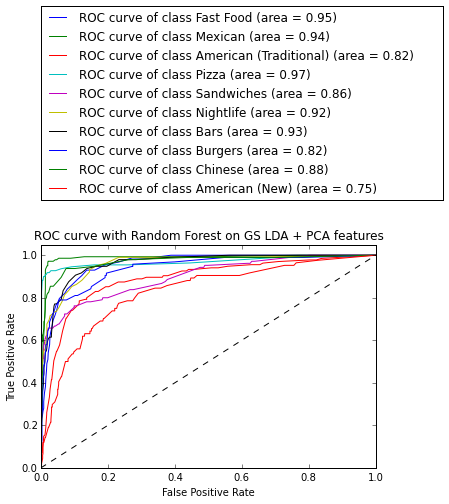
\includegraphics[scale=0.55]{img/roc_rf.png}
	\centering
	\caption{Roc curve for the Random Forest one-vs-all classifiers}
\end{figure}


\paragraph{Feature Importance}

\noindent Once we found a sufficiantly good estimator, we investigated the weights it assigned to each feature. This provided an answer to two important questions: \textit{Are the feature extracted from the reviews more relevant than the one provided by Yelp to classify the restaurants by category? Among the features extracted by the review, can we identify for each category one or several highly discriminative features?} Moreover, we can compare the performance of the two different LDA we used.\\

\noindent We answer these questions with a comparative study on four specific categories (Fast Food, Pizza, Nightlife and Bars) with a Random Forest on four kinds of features, depending on the type of LDA used and the reduction with PCA. The results with the features built with an NMF are similar to those with the OVI. We used the measure provided by scikit learn to evaluate the importance of the features. It is defined as the total decrease in node impurity averaged over all trees of the ensemble.

\begin{figure}[H]
\centering
\subfigure{
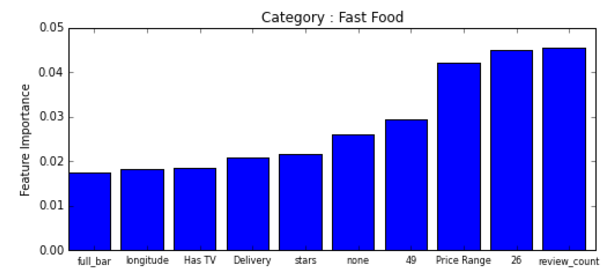
\includegraphics[scale=0.24]{img/fast_food_ovi.png}
}
\quad
\subfigure{
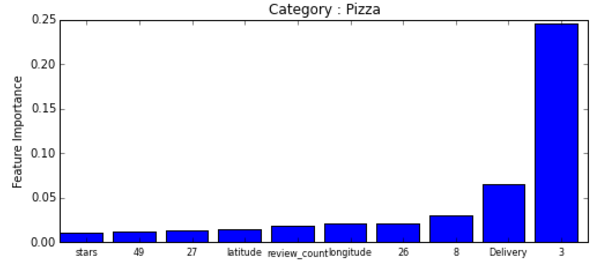
\includegraphics[scale=0.24]{img/pizza_ovi.png}
}
\subfigure{
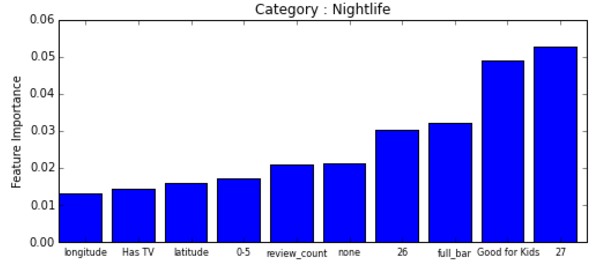
\includegraphics[scale=0.24]{img/nightlife_ovi.png}
}
\quad
\subfigure{
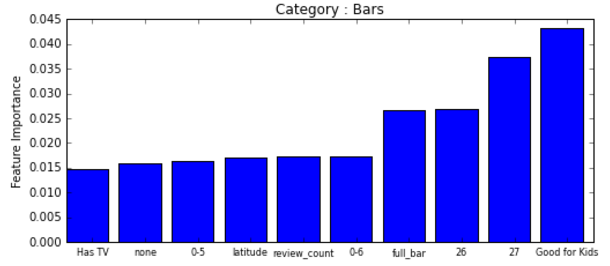
\includegraphics[scale=0.24]{img/bars_ovi.png}
}
%
\caption{Importance of the OVI LDA features in the one-vs-all Random Forest classification}
\label{fig:figure}
\end{figure}

\begin{figure}[H]
\centering
\subfigure{
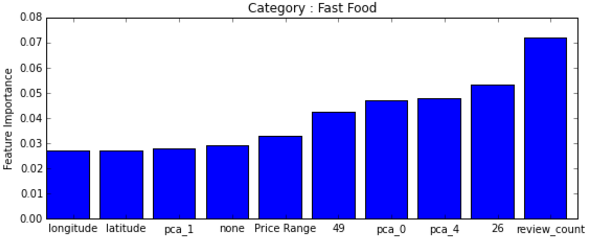
\includegraphics[scale=0.24]{img/fast_food_ovi_pca.png}
}
\quad
\subfigure{
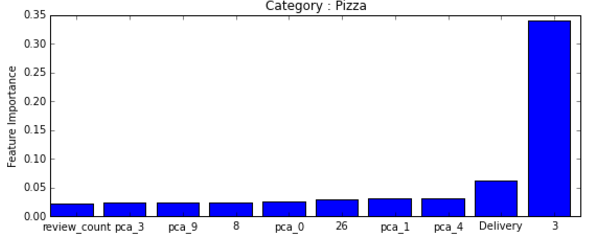
\includegraphics[scale=0.24]{img/pizza_ovi_pca.png}
}
\subfigure{
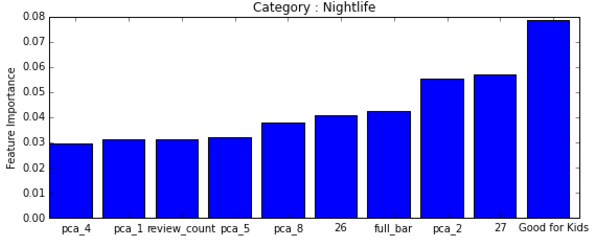
\includegraphics[scale=0.24]{img/nightlife_ovi_pca.png}
}
\quad
\subfigure{
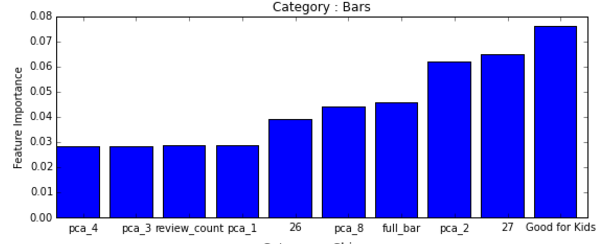
\includegraphics[scale=0.24]{img/bars_ovi_pca.png}
}
%
\caption{Importance of the OVI LDA features with PCA in the one-vs-all Random Forest classification}
\label{fig:figure}
\end{figure}

\begin{figure}[H]
\centering
\subfigure{
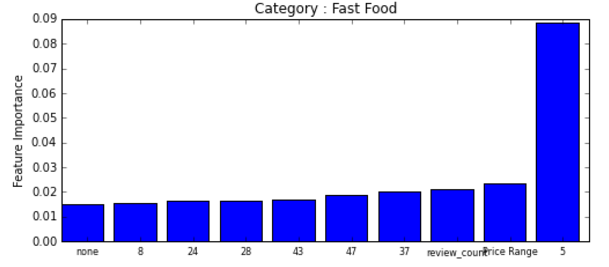
\includegraphics[scale=0.24]{img/fast_food_gs.png}
}
\quad
\subfigure{
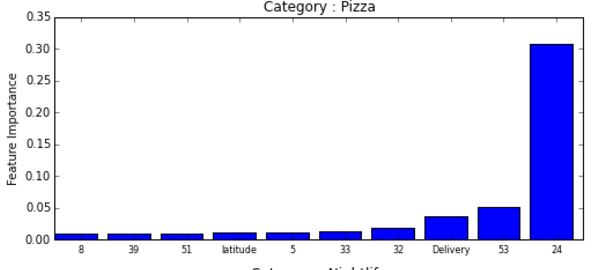
\includegraphics[scale=0.24]{img/pizza_gs.png}
}
\subfigure{
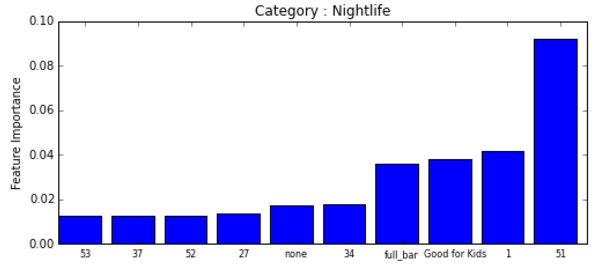
\includegraphics[scale=0.24]{img/nightlife_gs.png}
}
\quad
\subfigure{
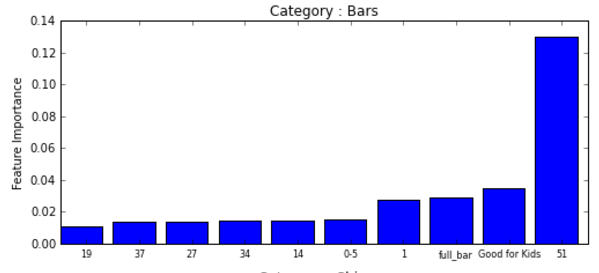
\includegraphics[scale=0.24]{img/bars_gs.png}
}
%
\caption{Importance of the GS LDA features in the one-vs-all Random Forest classification}
\label{fig:figure}
\end{figure}

\begin{figure}[H]
\centering
\subfigure{
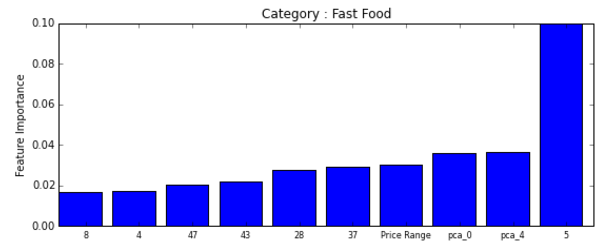
\includegraphics[scale=0.24]{img/fast_food_gs_pca.png}
}
\quad
\subfigure{
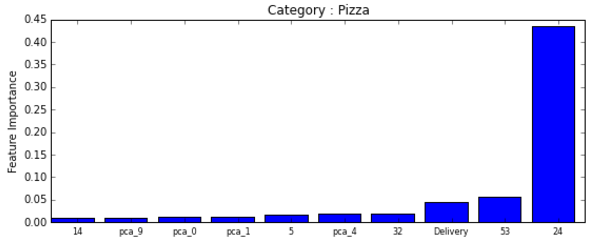
\includegraphics[scale=0.24]{img/pizza_gs_pca.png}
}
\subfigure{
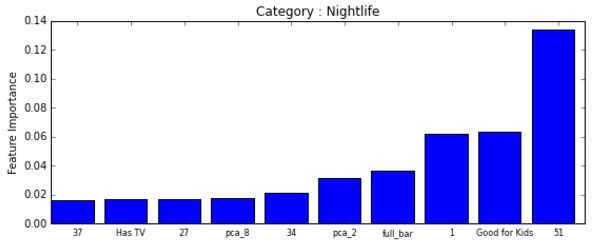
\includegraphics[scale=0.24]{img/nightlife_gs_pca.png}
}
\quad
\subfigure{
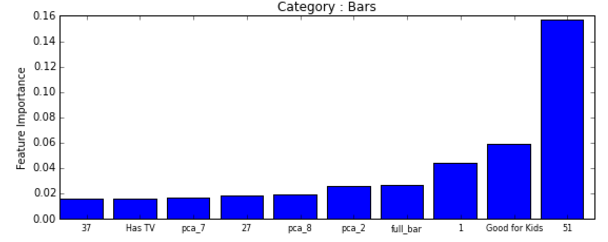
\includegraphics[scale=0.24]{img/bars_gs_pca.png}
}
%
\caption{Importance of the GS LDA features with PCA in the one-vs-all Random Forest classification}
\label{fig:figure}
\end{figure}

\begin{figure}[H]
\centering
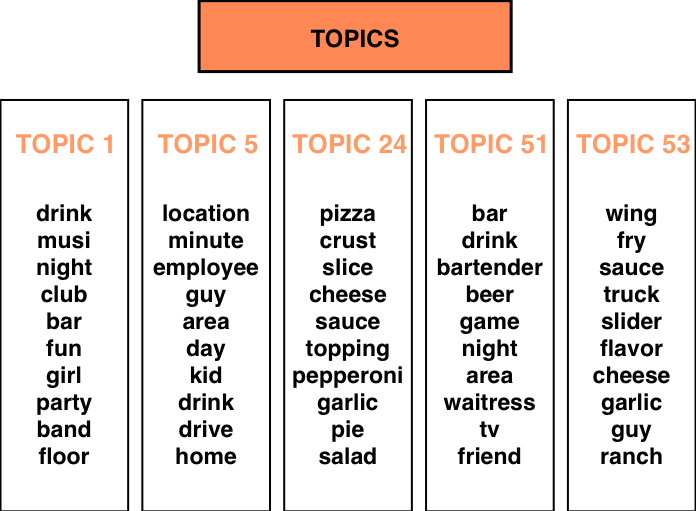
\includegraphics[width=1\linewidth]{img/gs_topics.png}
\caption{Topics extracted from the Las Vegas reviews using GS}
\end{figure}

\noindent First, considering the results for the OVI features, we observe that some properties provided by Yelp are discriminative for our classification. For example, the attribute \textit{Good for Kids} helps to sort the Bars and the Nightlife categories which is not surprising. The Fast Food may be the restaurants with the largest number of reviews as they have the largest number of customers, the model confirms this with the high weight on the \textit{reviews\_count}. This is also a cheap restaurant, hence the importance of the price range. As a result, it is worth considering the features provided by Yelp as they help discriminate the entries.\\

\noindent Second, for the Pizza category with the features extracted by the OVI we observe a discriminative feature which matchs the one about Pizza provided in the figure 3. Then, for the same LDA method, there is no discriminative feature for the other categories. Now, if we consider the results for the GS features, each category has a highly discriminative feature. Moreover, if we look at the most common words for each of these topics in the figure 10, we naturally understand their importance in the classification. This result confirms our analysis on the models. The Gibbs sampling method provides a finer topic distribution over the documents (here it is a label distribution over the restaurants).

\noindent Lastly, it is worth noticing the effect of the PCA on the feature importance. For both the OVI and the GS, if we look back at the Pizza category, the results with the PCA are much more clear-cut. The weight of the most important feature and its difference with those of the other features are higher. We can explain this by the fact that the projection gave more structure to the data and reduces the noise.\\

\noindent This part was about confronting our data to supervised methods to grasp their patterns and also coming up with a good classification. We provided empirical results to confirm the difference between the two common LDA methods and proved that with the Gibbs sampling, the LDA can be really efficient at finding the underlying topics on a set of documents.  It also proved that it performed much butter than a matrix factorization method. Related to our problem, it showed us that if numerical features provided by Yelp contained some information, the LDA features remained much more important when looking to find the labels of a restaurant.

\section{Unsupervised Clustering}
\subsection{Approach}

For this part of the project, we use the same features as for the supervised classification approach, i.e. the topic assignments. We wanted to see if it was possible to retrieve the original classification only based on the reviews. To do so and in order to check if our classification attempt was successful, we sampled about 1000 restaurants having tags in the following list of 6 categories: Sushi, Steakhouse, Seafood, Mexican, Sports and Breakfast \& Brunch. We then applied applied the following methodology.\\

Each restaurant is now represented as a probability distribution over the latent topics. Using the Shannon distance (symmetric Kullback-Liebler Divergence), we created a distance matrix gathering information on how close two restaurants are based on their reviews. After many experimentations, we chose to transform this distance matrix into a weighted adjacency matrix:\\

\begin{compactitem}
\item $w_{ij} = 5$ if $d_{Shannon}(r_i,r_j)<1$,
\item $w_{ij} = 0.1$ otherwise.\\
\end{compactitem}

\noindent The choice of having a non-zero weight between two restaurants even though they are not "close" is motivated by the fact that many graph clustering algorithm, in particular the WalkTrap algorithms that we used, only work on a connected graph.\\

\noindent We then transformed this adjacency matrix in an unweighted graph and applied the Walktrap algorithm for community detection.\\

\subsection{The WalkTrap Algorithm}
The WalkTrap Algorithm is a community detection algorithm created by Pascal Pons and Matthieu Latapy \cite{Gr}. The algortihm runs in time $O(n^2\log n)$ and space $O(n^2)$ where $n$ is the number of vertices in the graph. As mentioned in their paper, "the intuition behind the Walktrap is that random walks on a graph tend to get trapped into densely connected parts corresponding to communities".\cite{Gr} It relies on a new metric used to evaluate the distance between two vertices in a graph:
 $$r_{ij} = \sqrt{\sum\limits_{k=1}^{n}\frac{(P^t_{ik}-P^t_{kj})^2}{d(k)}}$$
 where $P^t_{ik}$ is the transition probability in $t$ steps and $d(k)$ is the degree of node k (number of edges incident to the vertex). We can then generalise this distance between two vertices to a distance between two communities. Using this distance, we can now apply a hierarchical clustering algorithm.

\begin{algorithm}[H]
\caption{Walktrap Algorithm}\label{euclid}
\begin{algorithmic}[1]
\State Start with a partition $\mathcal{P}_1=\{\{v\}, v \in V\}$
\State Compute the distances between all adjacent vertices
\While {$\mathcal{P}_t\neq V$}
\State Merge 2 communities $\mathcal{C}_i$ and $\mathcal{C}_j$ in $\mathcal{P}_k$ and create a new partition $\mathcal{P}_{k+1}$
\State Evaluate the distances between the communities in this new partition
\EndWhile
\end{algorithmic}
\end{algorithm}

\noindent The choice of communities to merge in step 4 is made using Ward's method. We look at minimising the mean within-cluster variance:
$$\frac{1}{n_\mathcal{C}}\sum\limits_{\mathcal{C}\in\mathcal{P}_{k}}\sum\limits_{i\in\mathcal{C}}r^2_{i\mathcal{C}},$$
\noindent where $n_\mathcal{C}$ is the number of communities at iteration $k$, and $r_{i\mathcal{C}}$ is the distance from vertex i to its community $\mathcal{C}$.\\

\subsection{Results}

We ran the algorithm from the \emph{igraph} \cite{igr} package in R on the three graphs generated with the three approaches mentionned above (NMF, OVI LDA, GS LDA). The results where extremely similar. We outputted a dendogram (cf. Annex) representing the obtained clustering. We colored the tag of each business for a better readability.  It is not yet entirely clear to us how to get the optimum number of clusters. We were puzzled to see that the Walktrap algorithm indicated that a cut into three big clusters represented the optimum partition. Knowing the structure of the sampled restaurants, we decided to further investigate the dendogram. As one can see on Figure 3, cutting the tree at different heights, we can obtain five clear colored communities, corresponding to five of the six tags we pre-selected.\\

\noindent We summarized this classification using a confusion matrix: 
\begin{figure}[H]
\centering
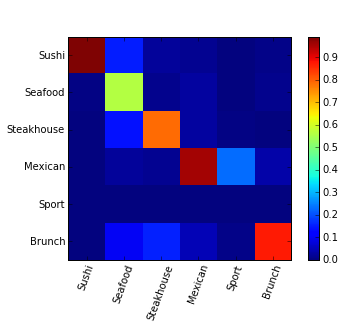
\includegraphics[width=1\linewidth]{img/confusion}
\caption{Confusion Matrix using the Walktrap Algorithm}
\end{figure}

\noindent With this method, we managed to detect 4 communities with great accuracy (over 80\%). Nevertheless, this classification still has some flaws and the most obvious one is the misclassification or even non-classification of the Sports bars (yellow). We focused a bit more on these venues and explored manually the tags associated with them. We noticed that these Sports bar have most of the time other tags such as "Restaurants","Bar", "American" and some even "Mexican". Reviews for these venues might have been misallocated due to the proximity of types of food, drinks or "ambiance" with Mexican restaurants. It is nonetheless interesting to note that they were grouped almost all together inside the Mexican restaurants, and that if we cut the tree at the sixth level then they would all be gathered in 2 cliques.\\

\noindent It seems that this method will succeed in making a difference between communities of restaurants if they are almost exlusive. It seems very unlikely to discover a restaurant that one can identify as both a Mexican and a Sushi place or even a Sushi place specialising in Breakfast (unless its speciality is the takagoyaki, a type of Japanese omelette made by "rolling together several layers of cooked egg"). It was often the case that misclassified restaurants had the tag "Buffet" which is for our purpose of classification our worst ennemy as it will phagocytose many categories at once.

\section{Next steps}

So far, we managed to extract the categories of the restaurants as latent features with a latent dirichlet allocation algorithm on the aggregated reviews for each restaurant. \\

Futur work could focus on the sub-cliques and try to get a finer classification by combining them with other features like check-ins, parking availability, etc. As a variant, we could also try a supervised LDA, where we use the existing categories as a response variable associated with each document and infer the joint model of the documents and the responses.\\

As a variant, we could try a supervised LDA, where we use the existing categories as a response variable associated with each document and infer the joint model of the documents and the responses. Lastly, this method is applicable on each review separately to predict the rating of the review, with a supervised lda also to avoid the predominance of the categories in the topics.


\section{conclusion}

This study illustrates different methods to extract feature from a set of documents. The results confirmed that the latent Dirichlet allocation manages to grasp the underlying features. The comparison with the supervised learning methods confirmed the importance of the feature extraction part in a machine learning problem. It also corroborates the assumption that the features of the businesses could be used to infer their category labels. Finally, the unsupervised clustering process we developped provides encouraging results and could result in an automation tool for Yelp to label properly its database. 

\section*{Code}

The code for this project can be found at the following address:

\begin{center}
www.github.com/nicodr/CS281
\end{center}


%----------------------------------------------------------------------------------------
%	REFERENCE LIST
%----------------------------------------------------------------------------------------

\nocite{*} % Insert publications even if they are not cited in the poster
\bibliographystyle{unsrt}
\bibliography{sample}
\end{multicols}

\newpage

\begin{figure*}
\centering

\includegraphics[angle=90,width=0.25\linewidth]{img/den_ovi2-1.png}
\caption{Dendogram outputted by the Walktrap Algorithm}
\end{figure*}

\end{document}



%----------------------------------------------------------------------------------------



